% Target: 8 pages with figures
\section{Osmotic Scaling and Scheduling}
In this section we describe our approach to scaling, and scheduling load balancer replicas, meaning the process by which we decide how many load balancer instances are in the system, and on which nodes they are placed.

\subsection{Osmotic scaler and scheduler}
To determine the number of replicas and their location we opted for an approach based on \textit{osmotic pressure}.
Like we outlined in previous chapters, osmotic pressure is a high level concept supposed to facilitate elastic diffusion, elastic diffusion being the process by which a central starting configuration, typically in the cloud, is extended to the edge dynamically based on request load with the goal of providing low latency communication for edge clients\cite{osmotic-middleware-rausch}. 
The general idea of this approach is that client requests generate pressure on nodes that are close to the clients, meaning that they could potentially host a load balancer instance, and then using this pressure in conjunction with a set threshold to determine both the number of load balancer instances and their locations.
If pressure at a node exceeds a certain level, because there are a lot of client requests originating close by, a load balancer will the, be placed at the node, thus lowering the pressure.
Conceptually this approach is supposed to create an equilibrium of pressure throughout the system, which results in a well-chosen set of load balancer instances.
This means that by using an osmotic approach, the scaling and scheduling decisions are effectively made together and cannot be controlled separately.

The main challenge of realizing an approach based on the concept of osmotic pressure is finding the method by which pressure is calculated. This can be particularly challenging when the system requires a manually set pressure threshold, since this requires the threshold value to fulfill a number of criteria:
\begin{enumerate}
    \item \textbf{Intuitive:} the threshold value should be at least somewhat intuitive to whoever determines it. It should be clear what a certain pressure threshold \textit{means}, and how it will affect the system.
    \item \textbf{Robustness:} the threshold should be reasonably robust to dynamically changing systems. A few extreme outliers in the system, for example extremely far or close nodes, should not require the threshold to be changed to still achieve the desired behaviour.
    \item \textbf{Linearity:} while not necessarily fully achievable, ideally changes in the threshold value should have a close to linear relationship with the scaling and scheduling behaviour. This is important in conjunction with its intuitiveness and is important to prevent sudden, unexpected effects such as dramatically changed system behaviour with minuscule changes in the threshold value.
\end{enumerate}

\subsection{Calculating osmotic pressure}
Building on the previously outlined requirements we can develop a pressure calculation methodology.
\subsubsection{Required data}
Because osmotic pressure based scaling and scheduling is at its core still a heuristic-driven approach, we cannot assume to have perfect global knowledge of the system.
Our approach is built with that in mind, staying close to assumptions about data availability already used for the load balancers themselves, and building on information current container orchestration platforms such as Kubernetes already provide.
For our calculation of osmotic pressure we require the following data:
\begin{itemize}
    \item Network locations of all function replicas, i.e. which nodes the instances are running on
    \item Network locations of all clients
    \item Number of all client requests, and which functions they are for
    \item Network locations of all load balancer replicas
    \item Network distances (latency) between nodes and clients
\end{itemize}
Replica information is readily available through state of the art container orchestration platforms, while network distances and exact client request numbers are relatively simple to obtain.
Because of this comparatively available set of data, we believe that our approach could easily be integrated into current serverless frameworks.
\subsubsection{Concept}
The basis of our pressure calculation is a hypothetical "what-if" scenario.
For all nodes in the system that could potentially host a load balancer, and are currently not doing so, we ask the question "what if there was a load balancer instance running on that node".
We then compare this hypothetical scenario to the current state of the system and determine whether the hypothetical addition of the load balancer on the node would constitute an improvement or deterioration in performance, and if so by how much.
For nodes that are hosting a load balancer already we do the same in reverse and ask "what if there wasn't a load balancer there", once again estimating whether performance would improve or deteriorate.

The two metrics we use to determine the impact of adding or removing load balancer replicas are the \textit{request share} and the \textbf{projected performance} of the node.
These metrics are calculated for each node on a per-function basis, and ultimately determine the pressure.

\subsubsection{Request Share}
\begin{figure}
    \centering
    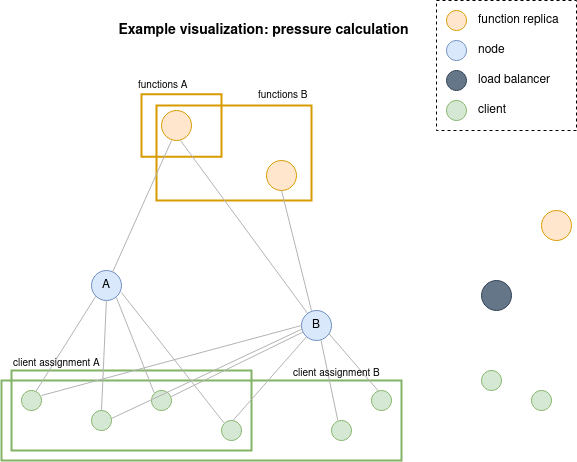
\includegraphics[width=12cm]{graphics/diagrams/client_lb_assignment.png}
    \caption{Assignment of clients and function replicas to potential load balancer nodes during pressure calculation}
    \label{fig:cl_lb_assignment}
\end{figure}
The request share is one of the central metrics we use to determine a node's pressure. In principle it shows which portion of the system's total incoming requests would be routed over that node, if it had a load balancer.
To calculate this value we need to first look at client assignment, meaning the process by which it is determined which client will send requests to which load balancer.

As we already outlined previously, one of our core assumptions is that clients will send their requests to whichever load balancer is closest from a network perspective, which is the load balancer with the shortest \gls{rtt}.
In keeping with our hypothetical scenario of "what if there was a load balancer on this node", clients will send their requests to this potential new load balancer if that node is closer to the clients than whichever load balancer instance is currently closest.
An example visualization of this client assignment for calculating request share can be seen in Figure \ref{fig:cl_lb_assignment}.
The specific number of clients our potential load balancer would service is, however, only of secondary importance. The more important and precise metric is the number of requests it will service.
We do not really care about whether there are a lot of clients sending few requests, or a low number of clients sending a large amount. What is important is only the number of requests going to the potential load balancer relative to the total amount sent.
Generally the data for this calculation is readily available, and can easily be gathered for example via existing load balancers reporting on the requests they receive.

A point to note here is that we only consider the requests sent within a certain time frame for this calculations, as they should be recent enough to be relevant for current scaling and scheduling decisions.
In our case we chose this time frame to be the last 60 seconds, which is relatively short but works within the relatively dynamic and heterogeneous systems we consider.
For real deployments this value might have to be adapted based on how dynamically the request load changes, how many requests each client typically sends in a session, and what amount of load is generally typical of the system.
The important point to consider here is that the time frame needs to be long enough to give a reasonably accurate picture, while not being so long that the data is delivers is not reflecting the current state of the system anymore.

Lastly, since there are multiple functions in the system, which we generally consider to be of equal importance, we calculate the request share the potential load balancer would receive on a per-function basis.
Thus we define the \textit{request share} as the following:
\[ \text{Let }N\text{ be the set of nodes,} \]
\[ L\text{ the set of nodes with running load balancer instances,} \]
\[ F\text{ the set of serverless functions,} \]
\[ \text{and }C\text{ the set of clients.} \]
\[ \text{Further let } dist(n,c) \text{ be the distance between a node } n \in N \text{ and client }c \in C\text{,}\]
\[ \text{ and let }requests(c, f) \text{ be the number of requests from client }c \in C \text{ for function }f \in F\]
\[ \text{Then for each node }n \in N\text{ the assigned clients are defined as} \]
\[ assignment(n) = \{c | c \in C \land dist(c,n) < min\{dist(l, c) | l \in L\}\}\]
\[ \text{Finally the request share for node } n \in N \text{ for function }f \in F \text{ is defined as } \]
\[ rqshare(n,f) = \frac{\sum_{c \in assignment(n)}requests(c,f)}{\sum_{c \in C}requests(c,f)}\]
Thus we define the request share of a node for a given function, as the fraction of all requests for that function the node would receive if it had a load balancer instance running.
\subsubsection{Projected Performance}
The second major metric that determines the pressure of a given node is what we refer to as the \textit{projected performance}.
This metric is once again based on the hypothetical scenario of "what if there was a load balancer on the given node" and is supposed to estimate the level of network performance we could expect if a load balancer is actually placed there.
Conceptually our notion of performance is rather simple.
It is determined by how close the clients are that would be assigned to that node, and by how close the function replicas are.
We once again calculate this metric for each node, and on a per-function basis.
To calculate the \textit{client distance} we use the average distance of all assigned clients, weighted by their relative share of requests among the assigned clients for the given function.

The calculation of the \textit{function distance} is somewhat more intricate.
Using a flat average over all function replicas is not a particularly suitable metric, since this would also consider the distance of function replicas that are far away, meaning that we would include the distance to function replicas we don't want the requests being sent to in the first place.
To address this issue we only consider a subsection of function replicas to calculate the function distance.
Our approach to the function distance is based on the assumption that the function scaling component correctly scales the function as required, meaning that we assume that the total number of function replicas is sufficient to serve the given number of incoming requests.
The number of function replicas we consider for a node is based on that nodes request share. We take into account the fraction of closest function replicas equal to the request share of the node for which we want to calculate the function distance.
If a node, for example, has a request share of 0.5, meaning 50\%, then its function distance is the average distance of the 50\% closest function replicas.
An example of this can once again be seen in Figure \ref{fig:cl_lb_assignment}, where nodes A and B have a differently sized share of functions assigned to them for distance calculation based on their respective request share.
Since we assume that the function replica scale is sufficient to handle the systems requests, this should mean that, not accounting for heterogeneity in function replica performance, the replicas considered for the function closeness metric are sufficient the incoming requests of the load balancer.
The reason we are not considering heterogeneity in replica performance is that this factor is not known beforehand, and in addition hard to estimate.
Finally we add the function distance and client distance together and invert them, since our subsequent calculations require the projected performance metric to have high values indicating good performance, and low values indicating poor performance.
Making this explicit we arrive at the following formulation for our projected performance:
\[\text{Let } replicas(f) \text{ be the set of replicas of a function }f \in F\]
\[\text{Then the client distance for a function }f \in F \text{ and node }n \in N \text{ is}\]
\[cldist(n,f) = \frac{\sum_{c \in assignment(n)}dist(n,c) \cdot requests(c,f)}{\sum_{c \in assignment(n)}requests(c,f)} \]
\[\text{Let }repdist_{n,f} = \langle r_{0}, r_{1}, ... \rangle \text{ be the list of replicas for a function }f \in F \text{ ordered by} \]
\[\text{their distance to }n \in N \text{ in ascending order such that for each pair } \]
\[(r_{i},r_{j}) \in repdist_{n,f}^{2}: i < j \implies dist(n, r_{i}) \leq dist(n, r_{j})\]
\[\text{Then the set of replicas considered is } \]
\[replicas(n,f) = \{r_{i} | r_{i} \in repdist_{n,f} \land i < \lfloor rqshare(n,f) \cdot |repdist_{n,r}| \rfloor\}\]
\[\text{Thus the function distance is }fndist(n,f) = \frac{\sum_{r \in replicas(n,f)}dist(n,f)}{|replicas(n,f)|} \]
\[\text{Finally the projected performance is }perf(n,f) = \frac{1}{cldist(n,f) + fndist(n,f)} \]
Needless to say slight adaptations of these formulas are necessary for a practical implementation.
For our simulator based evaluation the formulas are used exactly as we present them here, with the exception that special values are used as placeholders for undefined values, particularly those that result from a division by 0.
If a node has a request share of 0 for example, the projected performance is simply set to 0.
Likewise if the request share is > 0, the function distance calculation will take into account at least one replica, even if based on these formulas none would qualify.


\subsubsection{Pressure}
Now that we defined request shares and the projected performance we can move on to the actual pressure calculation.
In our approach we calculate what we call \textit{relative pressure}.
This means that the pressure of a given node is always in relation to the current state of the system, and not in absolutes.
This is done to ensure that the pressure calculation is not dependent on a-priori knowledge of the system.
If, for example, pressure were directly related to the number of requests per second the user would have to define what number of requests is considered high or low manually beforehand, negating precisely the kinds of advantage serverless frameworks are supposed to afford: Alleviating developers from complex configuration.

Our proposed notion of pressure is focused on the changes adding a load balancer on the node in question would bring to the system.
We start out by making an estimation of the average performance and impact of a load balancer in the system.
This notion of performance is based on the already described projected performance, and the load balancers request share.
We cannot rely purely on the projected performance, as it is also tremendously important for how many requests this performance is provided.
If we, for example, have a situation where we need to decide between two nodes which could potentially host a load balancer, that have a very high projected performance, then we most likely improve overall system performance more by selecting the node with the higher request share, since the high expected performance will affect more requests.

We call our estimation of the current system performance the \textit{status quo performance}.
To calculate it we once again rely on the projected performance, and the request share of node, although since we are interested in the current state of the system we consider these metrics only for nodes which currently host a load balancer.
The calculation of these metrics is exactly the same as for nodes that do not have load balancer instances deployed on them.
A slight difference to note is that the partition of clients onto nodes with load balancers will be without overlap, meaning that if we sum up all the request shares of a function over all nodes with a load balancer, the result would be 1, i.e. 100\%.

For our pressure metric this status quo performance is calculated using a weighted quantile.
The projected performance of the load balancer nodes are the values over which the quantile is calculated, while their respective request share is the weight.
We use the 50\% weighted quantile, also referred to as the weighted median, as our status quo performance.
In our testing the weighted median provided a robust metric that behaved predictably and similarly over different network topologies and cluster sizes.
It is, however, conceivable that there are situations in which this quantile should be set higher or lower depending on how dynamic the system changes, and how heterogeneous its structure and network topology are.
We should also note that at this point all of these metrics are still calculated on a per-function basis.
The values for each function are only combined at the very end, weighted by how important the individual functions are.
In our case the importance of individual functions is determined by which proportion of total requests are directed to it.
This means that we effectively treat each request as equally important and thus a function which gets double the traffic of another, for example, would also be considered twice as important when the individual function based metrics are combined.

% todo this should probably we rewritten a bit to be less repetitive
With this metric we can now calculate our pressure metric. For a given node we do this by calculating its impact on the system compared to the status quo performance.
Assuming that the status quo performance represents the current system performance overall, we compare the status quo performance with the performance of the system with the node added.
Since, as described earlier, the current set of load balancers services all client requests, adding a new load balancer will remove some of the traffic from existing load balancers.
This amount is represented by the potential load balancer node's request share.
To then calculate the system performance with the potential load balancer added we replace a part the size of the node's request share with the nodes performance.
Lastly we compare by how much adding a load balancer on this node changes the overall system performance, by calculating their difference in percent.
This percentage difference is the pressure value we use to make scaling and scheduling decisions in our osmotic system.
A positive pressure indicates that adding would likely improve performance, while negative pressure indicates that it would likely deteriorate overall system performance.
Thus we formally define our pressure as follows:
\[\text{For each function }f \in F \text{ it's relative importance is }\]
\[importance(f) = \frac{\sum_{c \in C}requests(c,f)}{\sum_{f' \in F}\sum_{c \in C}requests(c,f')} \]
\[\text{Let the set of tuples of a load balancer node's performance and request} \]
\[ \text{share for a function }f \in F \text{ be} \]
\[lbperf_{f} = \{(perf(l,f), rqshare(l,f)) | l \in L\} \]
\[\text{Then for a function the weighted median performance is } statusquo(f) = weightedmedian(lbperf_{f})\]
\[\text{Based on this we can estimate the system performance when adding a load balancer on node }n \in N\]
\[ addperf(n,f) = (rqshare(n,f) * perf(n,f)) + ((1 - rqshare(n,f)) * statusquo(f))\]
\[\text{which relative to the status quo performance gives us the pressure per function} \]
\[ fp(n, f) = \frac{addperf(n,f) - statusquo(f)}{statusquo(f)}\]
\[\text{Then combined the final pressure of the node is } p(n) = \sum_{f \in F}fp(n,f) \cdot importance(f)\]

\subsubsection{Downscaling Pressure}
Just like we need pressure to determine where load balancers should be scheduled, we also need to decide on conditions which trigger an existing load balancer to be removed.
Without this mechanic the osmotic scaling and scheduling component would not be able to properly adapt to changing system conditions, since load balancers that aren't placed effectively anymore cannot be removed.
During development we learned that an important property of the osmotic scaling and scheduling system is that it is consistent.
For our purposes this means that it should find a stable configuration eventually that doesn't change anymore unless the surrounding system parameters change.
In our testing the use of the exact same metric for removing load balancers as for adding them led to oscillations in their scheduling, meaning that there were cases were a load balancer would be added only to be removed again immediately.

To address this we use a slightly different measure of pressure for removing load balancer replicas.
It is also based on a hypothetical scenario, though in this case we try to estimate the consequences removing a load balancer would have on the system performance.
Compared to the pressure when adding load balancer replicas, we use a somewhat more accurate measure than for the removal process, since the original and future state of the system are more well known, considering it relies on more tangible and less hypothetical data.
First, the status quo before removal is calculated.
This is a weighted average of the projected performance of all load balancers weighted by their request share.
For the system performance once the load balancer is removed, we calculate how the system structure would change if the load balancer is removed.
The primary change this entails is that the removed load balancers clients would then send their requests to the next closest load balancer instance.
For simplicity and calculation efficiency, we assume that the clients would be assigned to whichever load balancer is closest to the one potentially getting removed.
At this point we recalculate the projected performance and request share of the load balancer that takes over the clients.
Based on this we can then calculate the system performance with the load balancer removed by again using a weighted average over the projected load balancer performances weighted by their request share, with the difference being that the load balancer we potentially remove is no longer counted, and its clients are moved to the next closest load balancer.
We then have an estimation of system performance with and without the load balancer in question, and go on to calculate their percentage difference.
This percentage difference tells us by how much removing the load balancer would affect overall system performance in percent, and based on a user defined threshold the scaler then decides to remove or keep each individual load balancer instance.
\[\text{For a function }f \in F \text{ the pre-removal status quo system performance is }\]
\[rmstatusquo(f) = \sum_{l \in L}perf(l,f) \cdot rqshare(l,f)\]
\[\text{If we then remove a load balancer }l \in L \text{ the clients are taken over by another load balancer} \]
\[l': dist(l,l') \leq min\{dist(l,l'') | l'' \in L \setminus \{l\}\} \implies assignment(l') = assignment(l') \cup assignment(l)\]
\[\text{Giving us the adapted set of load balancers }L' = L \setminus \{l\} \]
\[\text{Then the system performance without the load balancer for a function is} \]
\[rmperf(l,f) = \sum_{l' \in L'}perf(l',f) \cdot rqshare(l',f) \]
\[\text{Based on which we can calculate the removal pressure per function as}\]
\[ rmfp(l,f) = \frac{rmperf(l,f) - rmstatusquo(f)}{rmstatusquo(f)}\]
\[\text{and then combine them to the final removal pressure } rmp(l) = \sum_{f \in F}rmfp(l,f) \cdot importance(f)\]

\subsubsection{Throttled Scaling}
In our approach the scaling and scheduling components calculates pressures for all nodes and load balancers, and then makes subsequent scaling decisions, at a fixed interval.
While in theory multiple nodes could have a pressure beyond the set threshold that warrants adding a load balancer in a single interval, in our approach we artificially throttle this amount.
In our implementation of the scaling and scheduling component only a single load balancer can be added or removed per iteration.
We compensate for this comparatively slow rate of change by running the scaling and scheduling calculations at relatively short intervals.
There are two major reasons for our choice to limit the rate of change in the system in this way.

\begin{enumerate}
    \item The pressure metrics and calculation are based on the addition or removal of a single instance
    \item Since request shares potentially overlap, scheduling multiple load balancers often leads to immediate removal during the next scaling and scheduling cycle
\end{enumerate}

During development we observed faster convergence to a stable configuration when only adding or removing a single load balancer at a time.
We also considered changing our pressure calculations to optimize for a faster rate of change, but decided against it because these calculation are much less intuitive, which is detrimental to the ease of parametrization of the system, and most importantly the computational effort rises sharply with the number of load balancer instances that are considered simultaneously.
While the single node calculations we use only require calculating a maximum of 250 scenarios for a system with 250 nodes, the equivalent calculations for two nodes being scheduled simultaneously would require calculating up to 31125 scenarios for an equally sized system.
While this does limit the potential rate of change, we believe that a rate of change of about 4 load balancers per minute, which could still be increased if necessary, should be enough to handle the requirements of even comparatively dynamic systems.



